% !TeX root = Stageportfolio.tex



\begin{landscape}
	\subsubsection{Les 17-18}
	\begin{tabularx}{1.56\textwidth}{|p{0.35\textwidth}|X|}\hline
		\textbf{Administratieve gegevens}\newline\newline
		Kevin Truyaert\newline\newline
		technisch secundair onderwijs\newline
		3e graad, 1ste jaar, Techniek-Wetenschappen\newline
		VVKSO: \href{http://ond.vvkso-ict.com/leerplannen/doc/Toegepaste\%20fysica-2014-041.pdf}{http://ond.vvkso-ict.com/leerplannen /doc/Toegepaste\%20fysica-2014-041.pdf} \newline
		\underline{Lesonderwerp}:\newline Oefeningen op de algemene inductiewet \& Toepassingen op inductie & \textbf{Doelstellingen}
		\begin{itemize}[itemsep=0.08\baselineskip]
			\item B28: Met behulp van de wet van Lenz de zin van de inductiespanning vinden.
			\item B29: De algemene inductiewet hanteren.
			\item B30: Het werkingsprincipe van een generator weergeven.
			\item B31: De transformatorhouding bij de spanningen en de stromen van een ideale transformator toepassen en zijn functie bij het transport van elektrische energie toelichten.
		\end{itemize}
		\underline{Lesdoelen}\newline
		\vspace{-0.75cm}
		\begin{enumerate}[itemsep=0.08\baselineskip]
			\item De leerlingen reflecteren over het gemaakte labo.
			\item De leerlingen kunnen de wet van Faraday-Lenz op een rechte, bewegende geleider toepassen.
			\item De leerlingen kunnen de algemene inductiewet tijdens oefeningen hanteren.
			\item De leerlingen kunnen de werking van een wisselspanningsgenerator uitleggen.
			\item De leerlingen kunnen het doel van een transformator verwoorden.
		\end{enumerate} \\\hline
	\end{tabularx}\vfill \textcolor{white}{.} 


	\begin{tabularx}{1.56\textwidth}{|p{0.55\textwidth}|X|}
		\hline
		\multirow{2}{0.55\textwidth}{\textbf{Beginsituatie}\newline  
		Er zijn acht leerlingen binnen 5TW. Er heerst een algemene klassfeer. De leerlingen hebben al theorie gekregen rond en basisoefeningen gemaakt op elektromagnetische inductie. Ze zijn hier al vlot mee weg.  \newline\newline NOG AANVULLEN MET LERAARKENMERKEN.} & \textbf{Acties}\newline\newline  
		- Ik wil oefeningen op zo'n wijze brengen dat ze steeds dezelfde structuur hebben. Die structuur bouw ik eerst samen met de leerlingen op, om ze daarna zelfstandig aan de slag te laten gaan met oefeningen die steeds wat complexer worden. \PinkHighlight{Tijdens het zelfstandig maken van de oefeningen probeer ik toch zeker}{13cm} \PinkHighlight{de zwakkere leerlingen in de gaten te houden en hen individueler te coachen bij het}{15cm} \PinkHighlight{maken van oefeningen.}{4.5cm}
		\newline\newline\newline\newline\newline\newline\newline\newline
		
		\\ \cline{2-2}
		  & \textbf{Bronnen}\begin{itemize}
		  	\item Schramme, S. (2018-2019) Cursus hoofdstuk 5: elektromagnetische inductie
		  	\item Frederiksen (2014), Current Balance 4565.00
		  	\item Schramme, S. (2018-2019) Cursus hoofdstuk 6: toepassingen op inductie
		  	\item Giancoli, D. C. (2008). Physics for scientists and engineers. Pearson Education International.
		  \end{itemize}\\ \hline
	\end{tabularx}


\newpage


\begin{tabularx}{1.56\textwidth}{|p{1.5cm}|p{8cm}|X|p{4cm}|}
	\hline
	\textbf{Nr. lesdoel } & \textbf{Inhoud (timing)}  & \textbf{Organisatie } & \textbf{Media } \\ \hline
	1	&\underline{Bespreking Labo M4:} \underline{de stroombalans (10 minuten)}\newline
	Bespreken toekomstige aandachtspunten labo; waar gingen de leerlingen nu de mist in?
	&  \underline{Onderwijsleergesprek}\newline 
	\underline{Presentatie}
	\begin{itemize}
		\item Overlopen onderzoeksvragen
		\item Grootste aandachtspunten
		\begin{itemize}
			\item Eenheden!
			\item Grafiek: rechte door oorsprong
			\item Linken richtingscoëfficiënt met gemiddelde van F/...$\rightarrow$ indicatie fit
			\item Bepalen magnetische veldsterkte
		\end{itemize}
	\end{itemize}
	%De leerlingen krijgen hun door mij verbeterde labobundel terug en we overlopen de onderzoeksvragen van het labo nog even gezamenlijk. Ik vraag aan de leerlingen wat zij als essentie van het labo ervaren hebben. Vanuit dat standpunt wordt het labo besproken. Hierna wordt er niet meer terug gekomen op dit labo. Een duidelijk begrip van de Lorentzkracht is nodig voor de laatste twee hoofdstukken van magnetisme.
	&  Labobundel\newline\newline Slides (zie bijlage)
	\\ \hline
\end{tabularx}\vspace{5mm}
	
	\begin{tabularx}{1.56\textwidth}{|p{1.5cm}|p{6.5cm}|X|p{4cm}|}
		\hline
		\textbf{Nr. lesdoel } & \textbf{Inhoud (timing)}  & \textbf{Organisatie } & \textbf{Media } \\ \hline
		2\newline\newline3	&\underline{Oefeningen: de algemene} \underline{inductiewet (25 minuten)}\newline
			Oefeningen op Faraday-Lenz: Oefeningen 6, 7, 9 en 11 (8 als reserve)
		&  \underline{Zelfstandig oefeningen maken} \underline{Bespreking via correctiesleutel}\newline 
		- Leerlingen werken per twee\newline
			- Oefeningen maken terwijl ik observeer\newline
			- Leerlingen nemen zelf een oplossingssleutel (Met acht leerlingen kan ik in de gaten houden dat niemand zomaar een oplossingssleutel neemt)
		&   Cursus hoofdstuk 5 p15-16\newline\newline Krijtbord voor eventuele extra uitleg \newline\newline Correctiesleutels (4 per oefening)
		\\ \hline
	\end{tabularx}\vspace{5mm}



\begin{tabularx}{1.56\textwidth}{|p{1.5cm}|p{6.5cm}|X|p{4cm}|}
	\hline
	\textbf{Nr. lesdoel } & \textbf{Inhoud (timing)}  & \textbf{Organisatie } & \textbf{Media } \\ \hline
    4 & \underline{Werking wisselspanningsgenerator:} \underline{inleiding (5 minuten)}\newline
    	Opzet van de wisselspanningsgenerator verduidelijken en kennismaken met de werking ervan.
	&  \underline{Onderwijsleergesprek}\newline
	Projecteer wisselpanningsgenerator\newline
	Vraag leerlingen om alle componenten aan te duiden, te benoemen, \ldots 
	&  Cursus hoofdstuk 6 p6\newline\newline Slides om dit te schetsen
	\\ \hline
\end{tabularx}\vspace{5mm}


\begin{tabularx}{1.56\textwidth}{|p{1.5cm}|p{6.5cm}|X|p{4cm}|}
	\hline
	\textbf{Nr. lesdoel } & \textbf{Inhoud (timing)}  & \textbf{Organisatie } & \textbf{Media } \\ \hline
	4& \underline{Werking wisselspanningsgenerator:} \underline{eerste kwartdraai (8 minuten)}\newline
	De werking van de wisselspanningsgenerator verduidelijken: stap 1: eerste kwartdraai
	&  \underline{Onderwijsleergesprek}\newline  
	Werking van de algemene inductiewet is gekend\newline
	Eerste kwartdraai van de wisselspanningsgenerator samen bespreken. Zo vullen we samen het eerste kader op pagina 7 in.\newline
	\begin{itemize}
		\item Hoe verandert de hoek?
		\item Hoe verandert de flux hierdoor?
		\item Gevolg van die fluxverandering?
		\item Hoe is geïnduceerd magnetisch veld georiënteerd?
		\item Hoe loopt de inductiestroom doorheen de schakeling?
		\item Wat met de geïnduceerde spanning?
	\end{itemize}
	&  Cursus hoofdstuk 6 p7\newline\newline Krijtbord
	\\ \hline
\end{tabularx}\vspace{5mm}


\begin{tabularx}{1.56\textwidth}{|p{1.5cm}|p{6.5cm}|X|p{3cm}|}
	\hline
	\textbf{Nr. lesdoel } & \textbf{Inhoud (timing)}  & \textbf{Organisatie } & \textbf{Media } \\ \hline
	& \underline{Pauze (2 minuten)}\newline
	Even uitblazen tijdens het blokuur
	&  \underline{Pauze}\newline 
	&  
	\\ \hline
\end{tabularx}\vspace{5mm}


\begin{tabularx}{1.56\textwidth}{|p{1.5cm}|p{8cm}|X|p{4cm}|}
\hline
\textbf{Nr. lesdoel } & \textbf{Inhoud (timing)}  & \textbf{Organisatie } & \textbf{Media } \\ \hline
4& \underline{Werking wisselspanningsgenerator:} \underline{volgende kwartdraaien (5 minuten)}\newline
De leerlingen bepalen zelf het verloop van één van de andere kwartdraaien. 
&  \underline{Zelfstandig werk}\newline 
 - Per twee aan het werk (= 4 groepjes)\newline
 - Geef de leerlingen een getal (2, 3 of 4) $\rightarrow$ die kwartdraai uitwerken\newline
 - Indien klaar met hun kwartdraai$\rightarrow$ de volgende maken\newline
 - Ik geef de aanzet bij alle gevallen door de begin- en eindhoek te geven.
&  Cursus hoofdstuk 6 p7-8
\\ \hline
\end{tabularx}\vspace{5mm}

\begin{tabularx}{1.56\textwidth}{|p{1.5cm}|p{8cm}|X|p{4cm}|}
	\hline
	\textbf{Nr. lesdoel } & \textbf{Inhoud (timing)}  & \textbf{Organisatie } & \textbf{Media } \\ \hline
	4& \underline{Werking wisselspanningsgenerator:} \underline{volledige werking (15 minuten)}\newline
	De leerlingen overlopen het verloop van de wisselspanningsgenerator met elkaar. 
	&  \underline{Zelfstandig werk + onderwijsleergesprek}\newline  Ik laat verschillende leerlingen aan het woord om hun casus te bespreken en die te delen met hun medeleerlingen. Zo zal iedereen het volledige verloop beet hebben. Ik zorg dat iedere leerling aan bod gekomen is. Ik eindig met de werking van de wisselspanningsgenerator nog eens met een video samen te vatten.
	&  Cursus hoofdstuk 6 p7-8 \newline\newline Projectie
	\\ \hline
\end{tabularx}\vspace{5mm}



\begin{tabularx}{1.56\textwidth}{|p{1.5cm}|p{8cm}|X|p{4cm}|}
	\hline
	\textbf{Nr. lesdoel } & \textbf{Inhoud (timing)}  & \textbf{Organisatie } & \textbf{Media } \\ \hline
	4& \underline{Werking wisselspanningsgenerator:} \underline{verloop flux en inductiespanning} \underline{(8 minuten)}\newline
	Net volledige werking van de wisselspanningsgenerator doorlopen $\rightarrow$  Hoe verloopt de flux  en de inductiespanning in functie van de tijd?
	&  \underline{Zelfstandig werk + onderwijsleergesprek}\newline  
	- Projecteer startsituatie \newline
	- Vraag aan de leerlingen om in potlood enkele punten van de grafieken uit te zetten, vanuit de situaties die ze net gezien hebben (Iemand aan bord ook komen zetten?)\newline
	&  Cursus hoofdstuk 6 p9 \newline\newline Projectie\newline\newline Bord
	\\ \hline
\end{tabularx}\vspace{5mm}



\begin{tabularx}{1.56\textwidth}{|p{1.5cm}|p{8cm}|X|p{4cm}|}
	\hline
	\textbf{Nr. lesdoel } & \textbf{Inhoud (timing)}  & \textbf{Organisatie } & \textbf{Media } \\ \hline
	4& \underline{Werking wisselspanningsgenerator:} \underline{besluit(7 minuten)}\newline 
	Besluit vormen 
	&  \underline{Onderwijsleergesprek}\newline  
	- Hoe gebeurt de energieoverdracht?\newline - Wat is het verschil weer tussen een motor en een generator?
	&  Cursus hoofdstuk 6 p9-10 \newline\newline Projectie\newline\newline Bord
	\\ \hline
\end{tabularx}\vspace{5mm}




\begin{tabularx}{1.56\textwidth}{|p{1.5cm}|p{8cm}|X|p{4cm}|}
	\hline
	\textbf{Nr. lesdoel } & \textbf{Inhoud (timing)}  & \textbf{Organisatie } & \textbf{Media } \\ \hline
	5& \underline{Werking transformator:} \underline{inleiding (10 minuten)}\newline
	- Opbouw transfo\newline - Werking transfo
	&  \underline{Doceren}\newline 
	Eerder docerende manier van les geven (allemaal nieuwe zaken en begrippen) \newline
	- Transfo bouwen op tafel\newline
	- Benoemen onderdelen\newline
	- Begrippen linken met onderdelen
	Dit laatste stukje zal ik eerder op een docerende manier behandelen. De introductie van een transformator is niet eenvoudig, er zijn een heleboel componenten die benoemd moeten worden met de correcte terminologie (primaire - secundaire). Hierbij wil ik vooral spreken over de bouw en het doel van de transfo. Ik kies er hier voor om geen slot met herhaling van de les in te bouwen gezien er net de conclusie van de wisselspanningsgenerator gebeurd is. 	
	&  Cursus hoofdstuk 6 p11 \newline\newline Projectie\newline\newline Bord\newline\newline Materiaal transfo: spoelen, en ijzeren U.
	\\ \hline
\end{tabularx}\vspace{5mm}




	
\end{landscape}


%\subsection*{Bijlage 5.1: slides introductie}

%
%\subsection*{Bijlage 1.2: bordschema theorie}
%\begin{center}
%	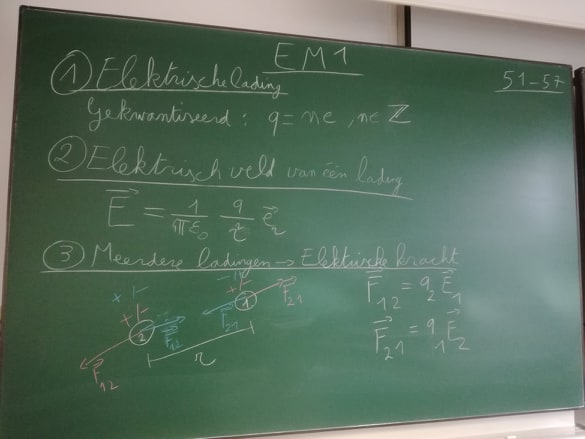
\includegraphics[width=0.9\textwidth]{Bord1a}
%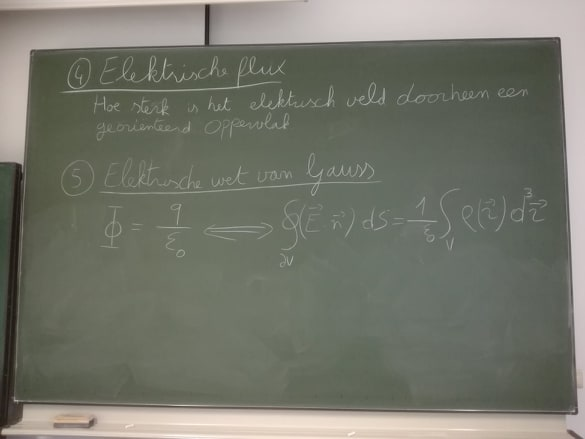
\includegraphics[width=0.9\textwidth]{Bord1b}
%\end{center}
%\newpage
%
%
%\includepdf[scale = 0.8,pages = 17,pagecommand=\subsection*{Bijlage 1.3: opgeloste oefeningen}]{Observaties_OpgelosteOef}
%\includepdf[scale = 0.8,pages =18-20,pagecommand=]{Observaties_OpgelosteOef}
%
%
%
%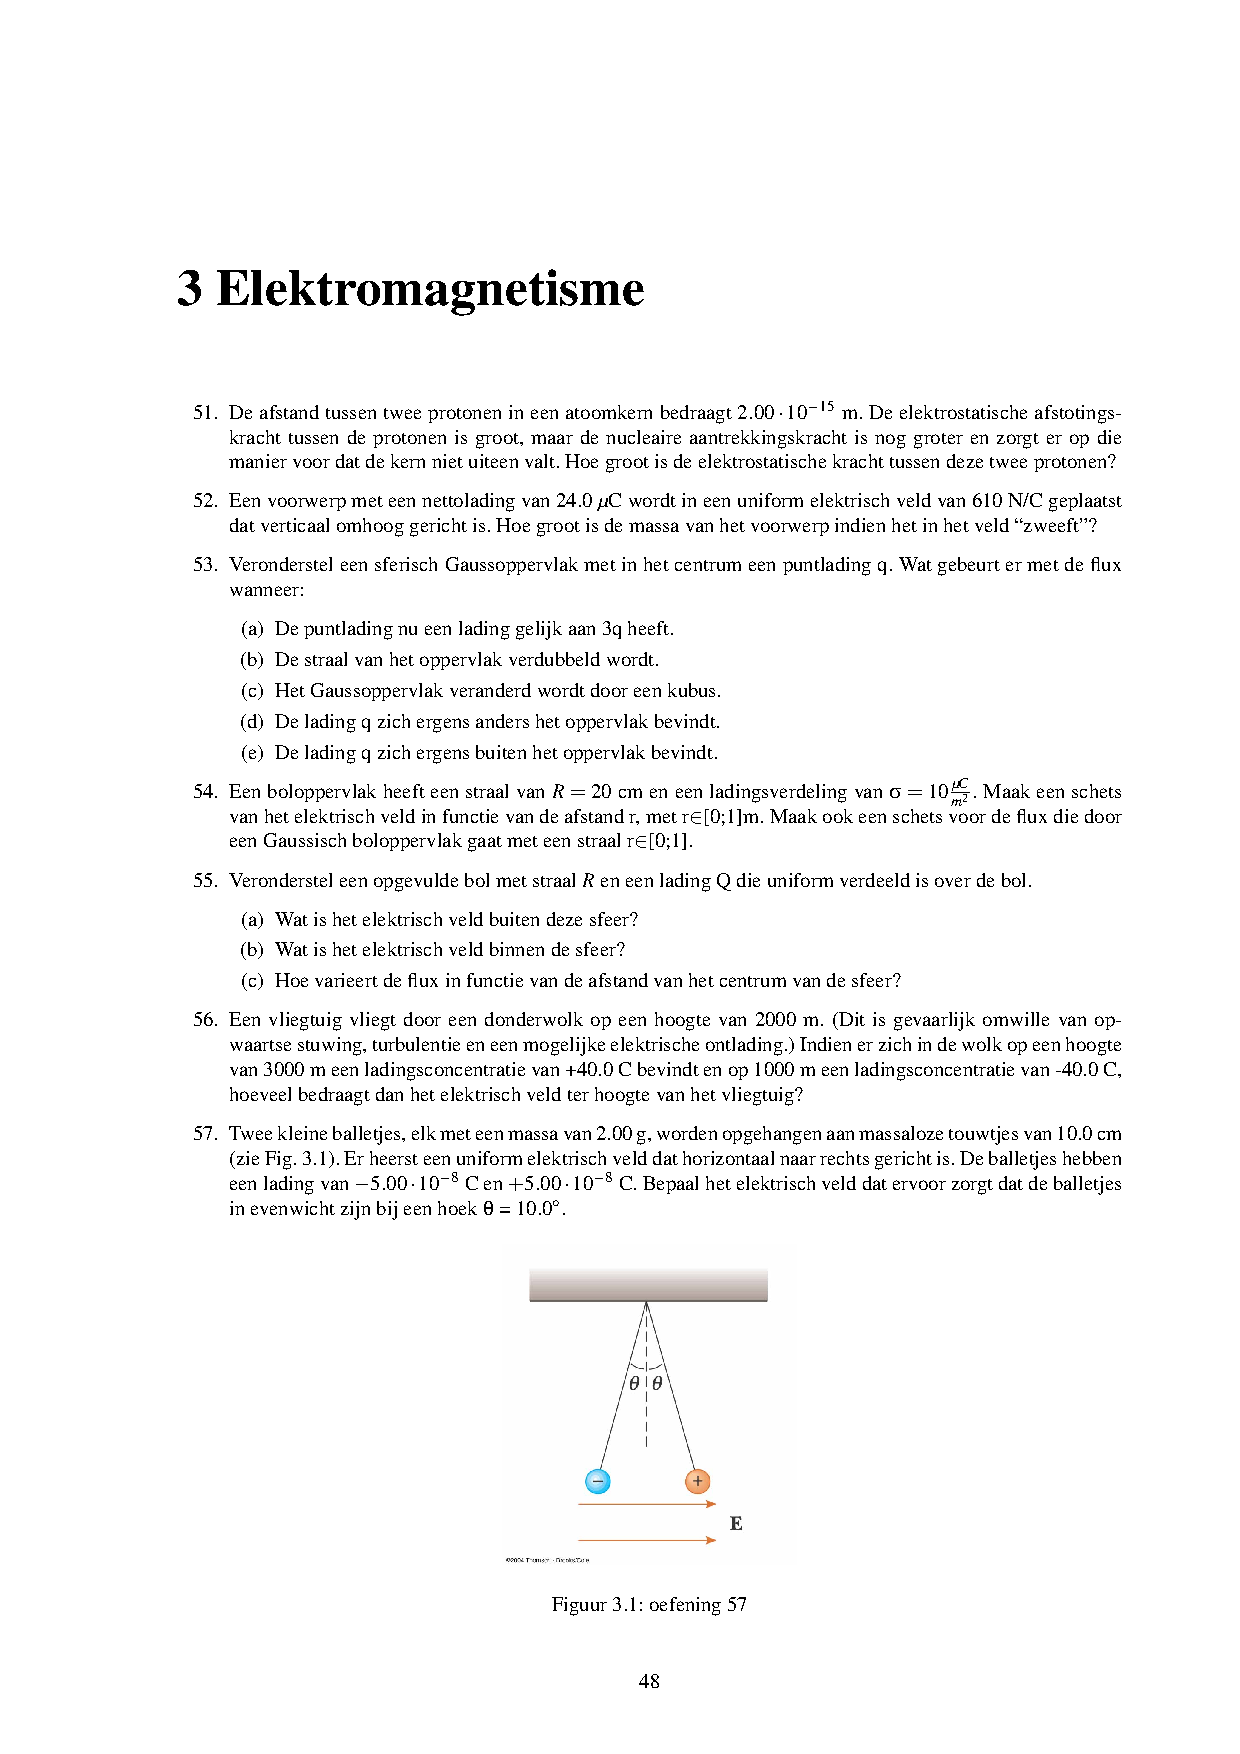
\includepdf[scale = 0.95,pages = 1,pagecommand=\subsection*{Bijlage 1.4: oefeningenbundel elektromagnetisme}]{OefeningenBundel}
%\includepdf[scale = 0.95,pages =2-,pagecommand=]{OefeningenBundel}